\documentclass[tikz,crop]{standalone}

\usepackage[T1]{fontenc}
\usepackage[tt=false,type1=true]{libertine}
\usepackage[varqu]{zi4}
\usepackage{newtxmath}
\usepackage[dvipsnames]{xcolor}
\usepackage{tikz}
\usepackage{marvosym}
\usepackage[marvosym]{tikzsymbols}
\usetikzlibrary{arrows, matrix, arrows.meta, shapes, shapes.arrows, shapes.multipart, shapes.symbols, fadings, fit, positioning, decorations.pathreplacing, angles, quotes}

\begin{document}
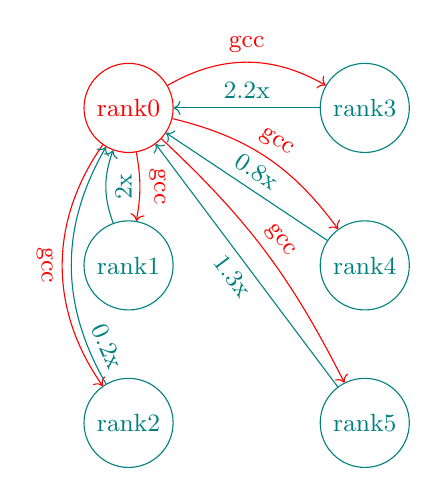
\begin{tikzpicture}[teal,
  decoration={random steps,segment length=1mm,amplitude=0.2pt},
  every node/.style={draw}, align=center, font=\small,
  every edge/.style={draw, ->},
]
\node[circle,red] at (0,0)  (rank0) {rank0};
\node[circle] at (0,-2) (rank1) {rank1};
\node[circle] at (0,-4) (rank2) {rank2};
\node[circle] at (3,0)  (rank3) {rank3};
\node[circle] at (3,-2) (rank4) {rank4};
\node[circle] at (3,-4) (rank5) {rank5};
\path
(rank0) edge[red, bend left=10] node[above, sloped, draw=none]{gcc} (rank1)
(rank1) edge[bend left=20] node[below, sloped, draw=none]{2x} (rank0)

(rank0) edge[red, bend right=35] node[sloped, below, draw=none]{gcc} (rank2)
(rank2) edge[bend left=30] node[very near start, sloped, above, draw=none]{0.2x} (rank0)

(rank0) edge[red, bend left] node[above, draw=none]{gcc} (rank3)
(rank3) edge[] node[above, draw=none]{2.2x} (rank0)

(rank0) edge[red, bend left=20] node[above, sloped, draw=none]{gcc} (rank4)
(rank4) edge[] node[above, sloped, draw=none]{0.8x} (rank0)

(rank0) edge[red, bend left=10] node[above, sloped, draw=none]{gcc} (rank5)
(rank5) edge node[below, sloped, draw=none]{1.3x} (rank0)
;
\end{tikzpicture}
\end{document}
